% ============================================================
% EXPERIMENTS
% ============================================================

\section{Experiments}
\label{sec:experiments}

This section describes our experimental setup and presents the results of our comparative evaluation. We detail the dataset construction (\Cref{sec:dataset}), evaluation metrics (\Cref{sec:metrics}), hyperparameter selection process (\Cref{sec:hyperparameters}), and present the main results (\Cref{sec:results}).

% ------------------------------------------------------------
\subsection{Dataset}
\label{sec:dataset}
% ------------------------------------------------------------

We construct a comprehensive cryptocurrency dataset spanning over seven years of market data.

\paragraph{Data Source.} Daily OHLCV (Open, High, Low, Close, Volume) data is collected from Binance via the CCXT library. The dataset covers 37 unique cryptocurrencies, with daily availability varying between 8 and 35 assets depending on index membership and cold-start eligibility requirements.

\paragraph{Temporal Splits.} We partition the data into non-overlapping periods following walk-forward evaluation principles~\citep{lucarelli2020dqlcrypto}:

\begin{table}[htbp]
\centering
\caption{Dataset temporal splits. The warmup period builds initial lookback windows. Development data is used for training and hyperparameter selection. Test data is strictly held out for final evaluation.}
\label{tab:splits}
\begin{tabular}{llrl}
\toprule
\textbf{Split} & \textbf{Period} & \textbf{Days} & \textbf{Purpose} \\
\midrule
Warmup & 2018-07-01 $\rightarrow$ 2018-08-31 & 62 & Build 60-day lookback \\
Train (train\_core) & 2018-09-01 $\rightarrow$ 2023-06-30 & 1,848 & Agent training \\
Validation & 5 regime windows & ${\sim}$100 & Hyperparameter selection \\
Test & 2024-01-01 $\rightarrow$ 2025-10-31 & 646 & Out-of-sample evaluation \\
\bottomrule
\end{tabular}
\end{table}

\paragraph{Regime-Based Validation.} Rather than using a single contiguous validation period, we carve out five approximately 20-day windows corresponding to qualitatively distinct market regimes. These include the late 2018 cryptocurrency winter (val\_2018\_crash), the March 2020 COVID-induced market crash (val\_covid), the 2021 bull market (val\_bull), the 2022 deleveraging period (val\_bear), and the 2023 low-volatility consolidation (val\_chop). This regime-diverse validation strategy prevents overfitting hyperparameters to a single market condition~\citep{jiang2016drlt, jiang2017eIIE}, ensuring that selected configurations generalize across bull markets, bear markets, and high-volatility crash periods alike.

% ------------------------------------------------------------
\subsection{Evaluation Metrics}
\label{sec:metrics}
% ------------------------------------------------------------

We evaluate portfolio performance using standard metrics from quantitative finance, encompassing return measures, risk metrics, and trading activity indicators.

\paragraph{Return Metrics.} Cumulative return measures the total percentage gain over the evaluation period, providing an absolute performance benchmark. We also report the Compound Annual Growth Rate (CAGR), which annualizes returns while properly accounting for compounding effects, enabling comparison across periods of different lengths.

\paragraph{Risk-Adjusted Performance.} The Sharpe ratio~\citep{sharpe1966mutual} quantifies risk-adjusted return as the ratio of annualized excess return to annualized volatility, assuming a zero risk-free rate given the cryptocurrency context. We complement this with the Sortino ratio, which penalizes only downside volatility by using only negative returns in the denominator, providing a measure more aligned with investor preferences. Maximum drawdown captures the largest peak-to-trough decline observed during the evaluation period, representing worst-case loss exposure. The Calmar ratio, computed as CAGR divided by maximum drawdown, combines these perspectives into a single efficiency metric.

\paragraph{Trading Activity.} Portfolio turnover, defined as the mean daily $L_1$ norm of weight changes $\|\vect{w}_t - \vect{w}_{t-1}\|_1$, quantifies trading activity. High turnover strategies incur greater transaction costs, making this metric essential for assessing practical viability in markets with non-trivial trading frictions.

% ------------------------------------------------------------
\subsection{Hyperparameter Selection}
\label{sec:hyperparameters}
% ------------------------------------------------------------

We employ Bayesian hyperparameter optimization using Optuna~\citep{optuna2019} to efficiently search the high-dimensional configuration space.

\paragraph{Search Protocol.} For the value-based DQN and DDQN agents, we use the Tree-structured Parzen Estimator (TPE) sampler to guide the search over 50 candidate configurations. Each configuration is evaluated by training for 50 episodes using 100-day sliding windows sampled from the training period, followed by validation across five episodes on the regime-diverse validation windows with a fixed random seed for reproducibility. The optimization objective maximizes mean validation return, with MedianPruner providing early termination for unpromising trials. We additionally implement Q-value explosion detection, terminating any trial where mean Q-values exceed 10,000 to prevent numerical instability from wasting computational resources.

\paragraph{Search Space.} The hyperparameter ranges explored are shown in \Cref{tab:search_space}. The discount factor $\gamma$ spans from 0.5 to 0.99, accommodating both short-horizon and long-horizon reward weighting. Learning rates are sampled log-uniformly between $10^{-5}$ and $10^{-3}$ to cover several orders of magnitude. Architectural choices include batch sizes of 32, 64, or 128, replay buffer capacities of 10,000 or 50,000 transitions, and network hidden dimensions ranging from two-layer configurations ([128, 64]) to deeper three-layer architectures ([512, 256, 128]). Exploration parameters include $\epsilon$ decay schedules of 300, 500, or 1,000 episodes and terminal $\epsilon$ values between 0.01 and 0.1.

\begin{table}[htbp]
\centering
\caption{Hyperparameter search space for DQN/DDQN agents.}
\label{tab:search_space}
\begin{tabular}{lll}
\toprule
\textbf{Hyperparameter} & \textbf{Range} & \textbf{Scale} \\
\midrule
Discount factor ($\gamma$) & $[0.5, 0.99]$ & Uniform \\
Learning rate & $[10^{-5}, 10^{-3}]$ & Log-uniform \\
Batch size & $\{32, 64, 128\}$ & Categorical \\
Replay buffer size & $\{10{,}000, 50{,}000\}$ & Categorical \\
$\epsilon$ decay episodes & $\{300, 500, 1000\}$ & Categorical \\
$\epsilon$ final & $[0.01, 0.1]$ & Uniform \\
Target update frequency & $\{50, 100, 200\}$ & Categorical \\
Hidden dimensions & $\{[128,64], [256,128], [512,256,128]\}$ & Categorical \\
\bottomrule
\end{tabular}
\end{table}

\paragraph{Training Protocol.} Using the best hyperparameters identified through the search, we train the final models with extended episode budgets. DQN trains for 400 episodes and DDQN for 300 episodes, both using 100-day sliding windows sampled from the training period. The REINFORCE agent, contributed as a separate implementation with independent tuning, trains for 10,000 episodes. All agents employ early stopping with patience of 5 validation checks (performed every 50 episodes for value-based methods) to prevent overfitting, and we checkpoint the best model based on mean validation return for final evaluation.

% ------------------------------------------------------------
\subsection{Results}
\label{sec:results}
% ------------------------------------------------------------

We evaluate all six strategies on the held-out test period (January 2024 -- October 2025, 646 trading days). Results are summarized in \Cref{tab:main_results} and visualized in Figures~\ref{fig:cumulative_returns}--\ref{fig:allocation_comparison}.

% Main results table
\begin{table}[htbp]
\centering
\caption{Test set performance comparison across all agents and baselines. Best values in \textbf{bold}, second-best \underline{underlined}. Test period: January 2024 -- October 2025 (646 trading days).}
\label{tab:main_results}
\begin{tabular}{lcccccc}
\toprule
\textbf{Agent} & \textbf{Return (\%)}  & \textbf{CAGR (\%)} & \textbf{Sharpe} & \textbf{Sortino} & \textbf{Max DD (\%)} & \textbf{Turnover (\%)} \\
\midrule
\multicolumn{7}{l}{\textit{Baselines}} \\
Equal Weight     & \underline{168.50} & \underline{74.88} & 1.217 & 1.250 & 48.87 & \textbf{0.25} \\
Market Cap       & 159.30 & 71.46 & \underline{1.240} & \underline{1.298} & \underline{44.17} & 0.34 \\
Mean-Variance    & \textbf{366.54} & \textbf{139.07} & \textbf{1.640} & \textbf{1.691} & \textbf{39.96} & 13.50 \\
\midrule
\multicolumn{7}{l}{\textit{RL Agents}} \\
DQN              & 155.47 & 70.03 & 1.146 & 1.175 & 52.59 & 10.88 \\
DDQN             & 144.50 & 65.85 & 1.135 & 1.157 & 52.56 & 8.39 \\
REINFORCE        & 166.98 & 74.32 & 1.212 & 1.247 & 48.72 & 0.82 \\
\bottomrule
\end{tabular}
\end{table}

% Cumulative returns figure
\begin{figure}[htbp]
    \centering
    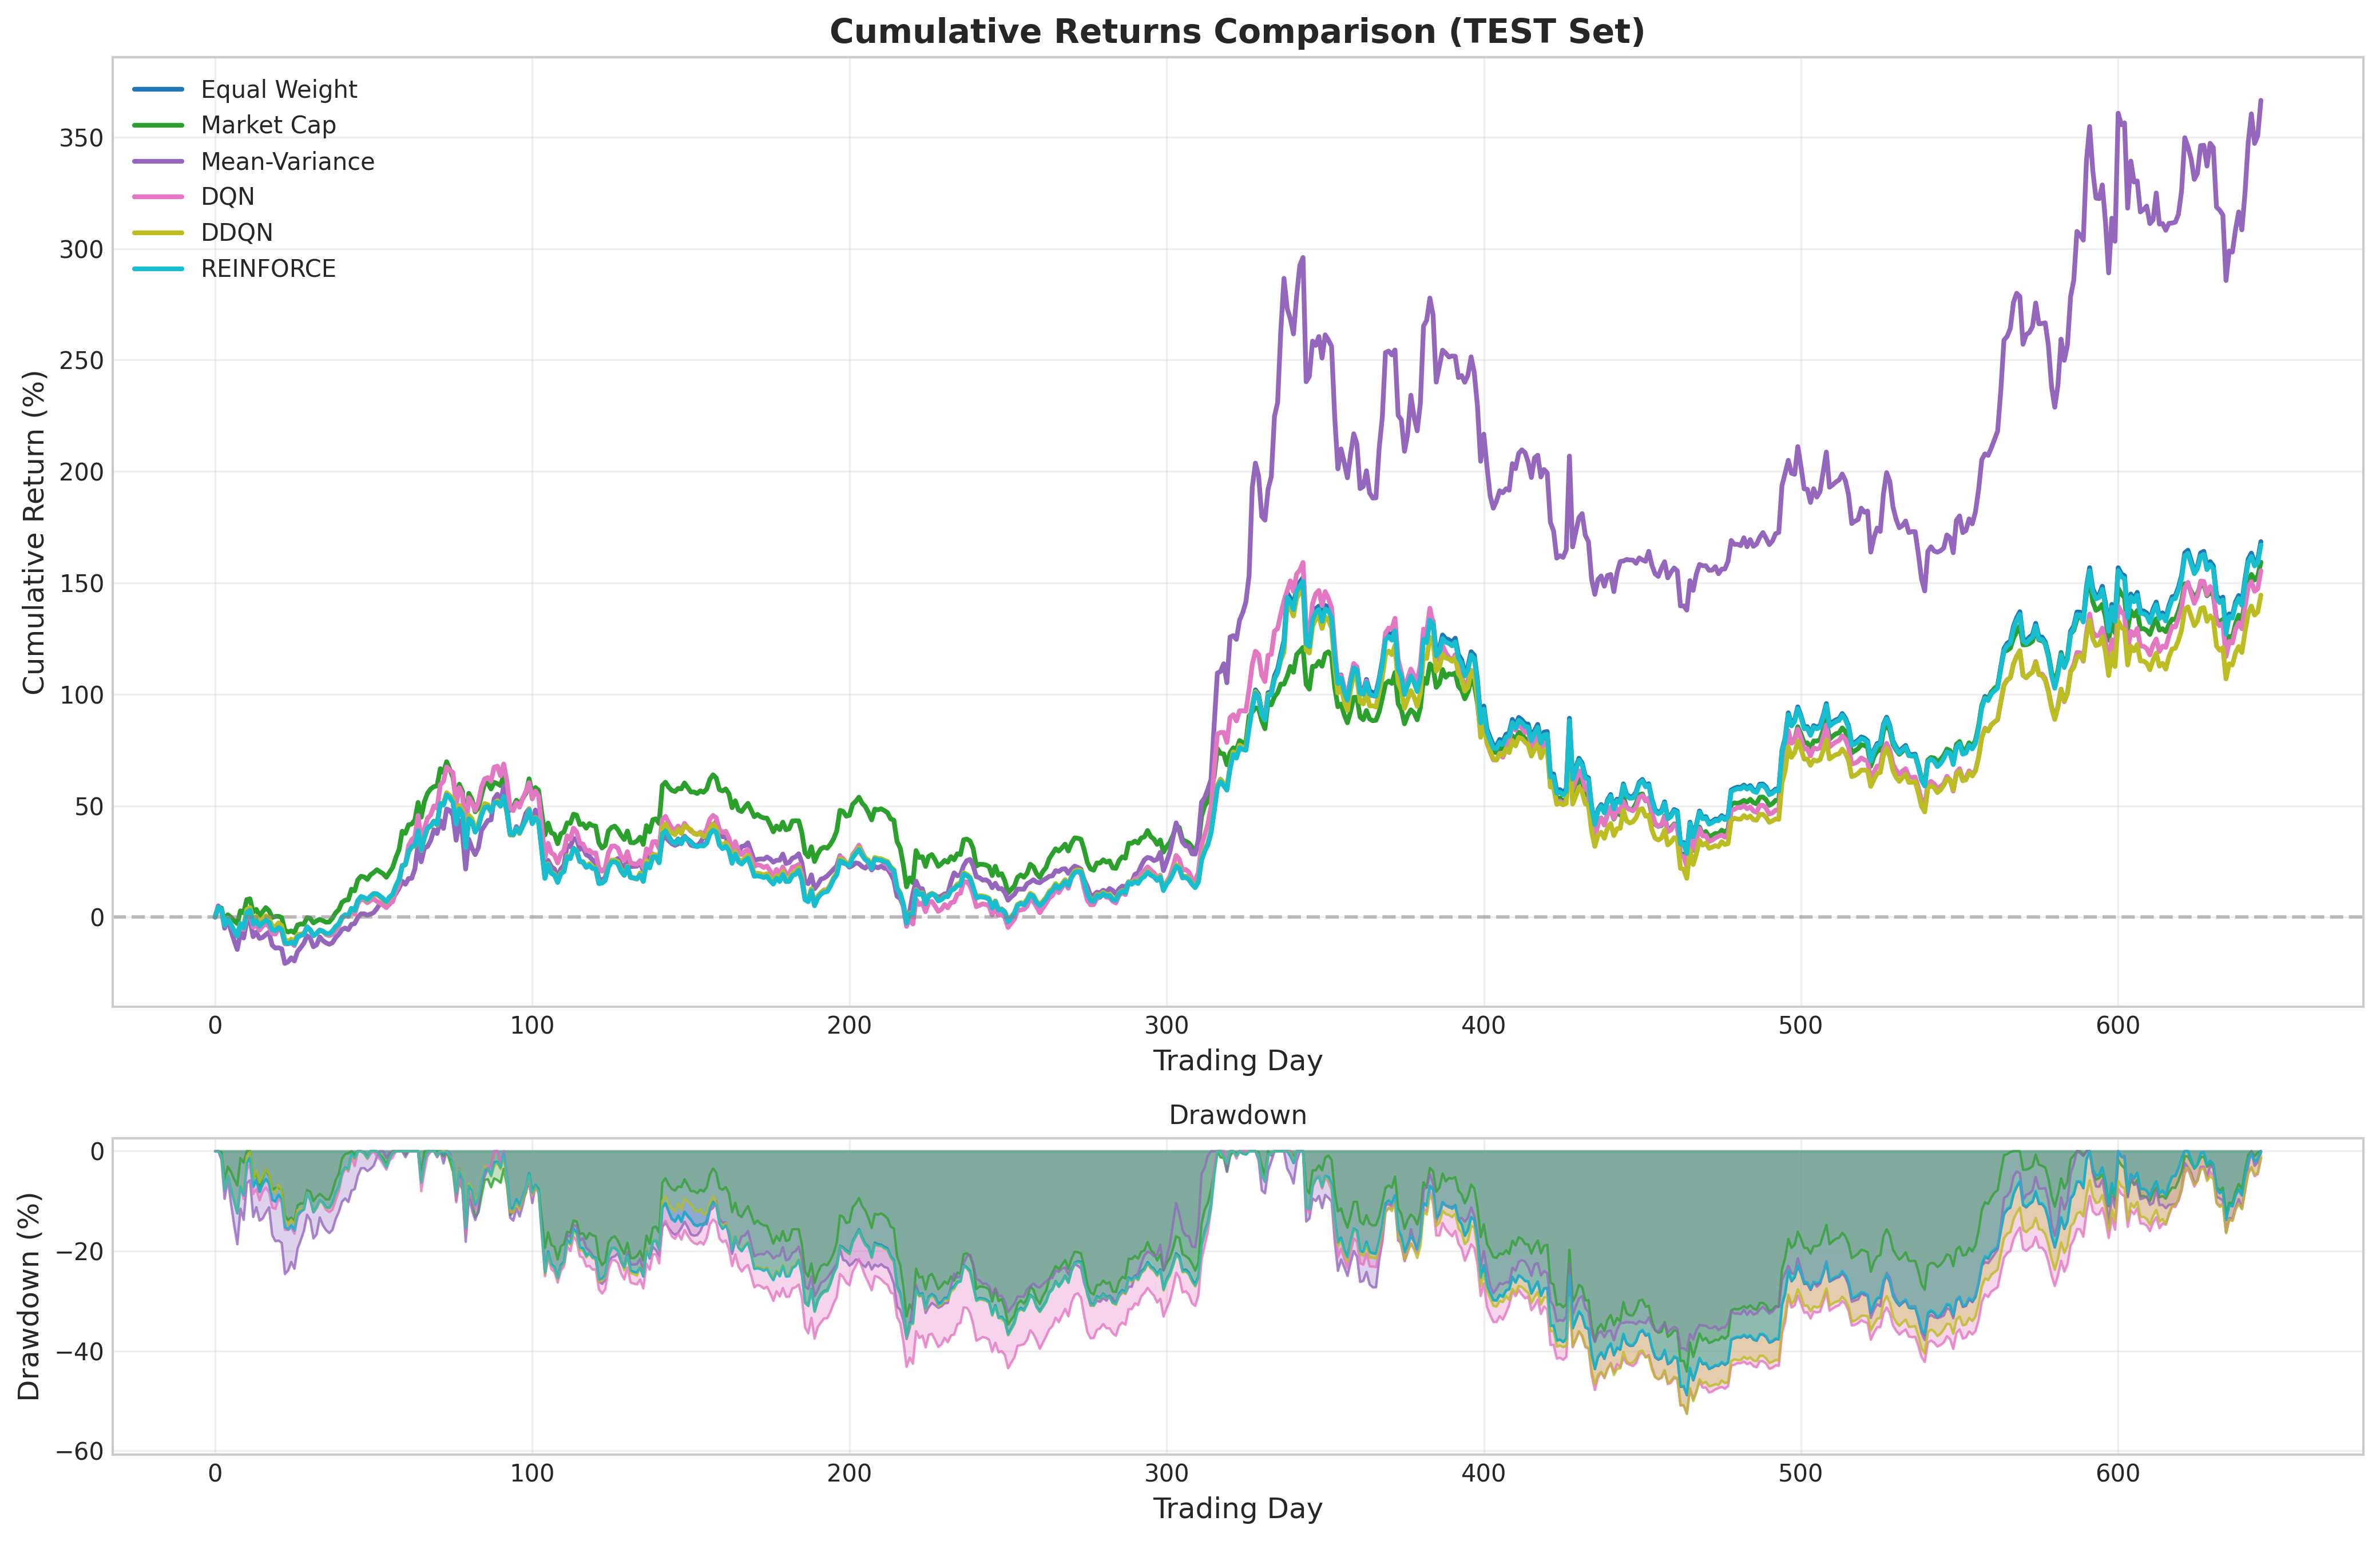
\includegraphics[width=\textwidth]{figures/cumulative_returns.png}
    \caption{Cumulative returns over the test period (January 2024 -- October 2025). Mean-Variance optimization substantially outperforms all other strategies, achieving 366\% cumulative return. The three RL agents (DQN, DDQN, REINFORCE) perform comparably to the Equal Weight baseline.}
    \label{fig:cumulative_returns}
\end{figure}

% Drawdown figure
\begin{figure}[htbp]
    \centering
    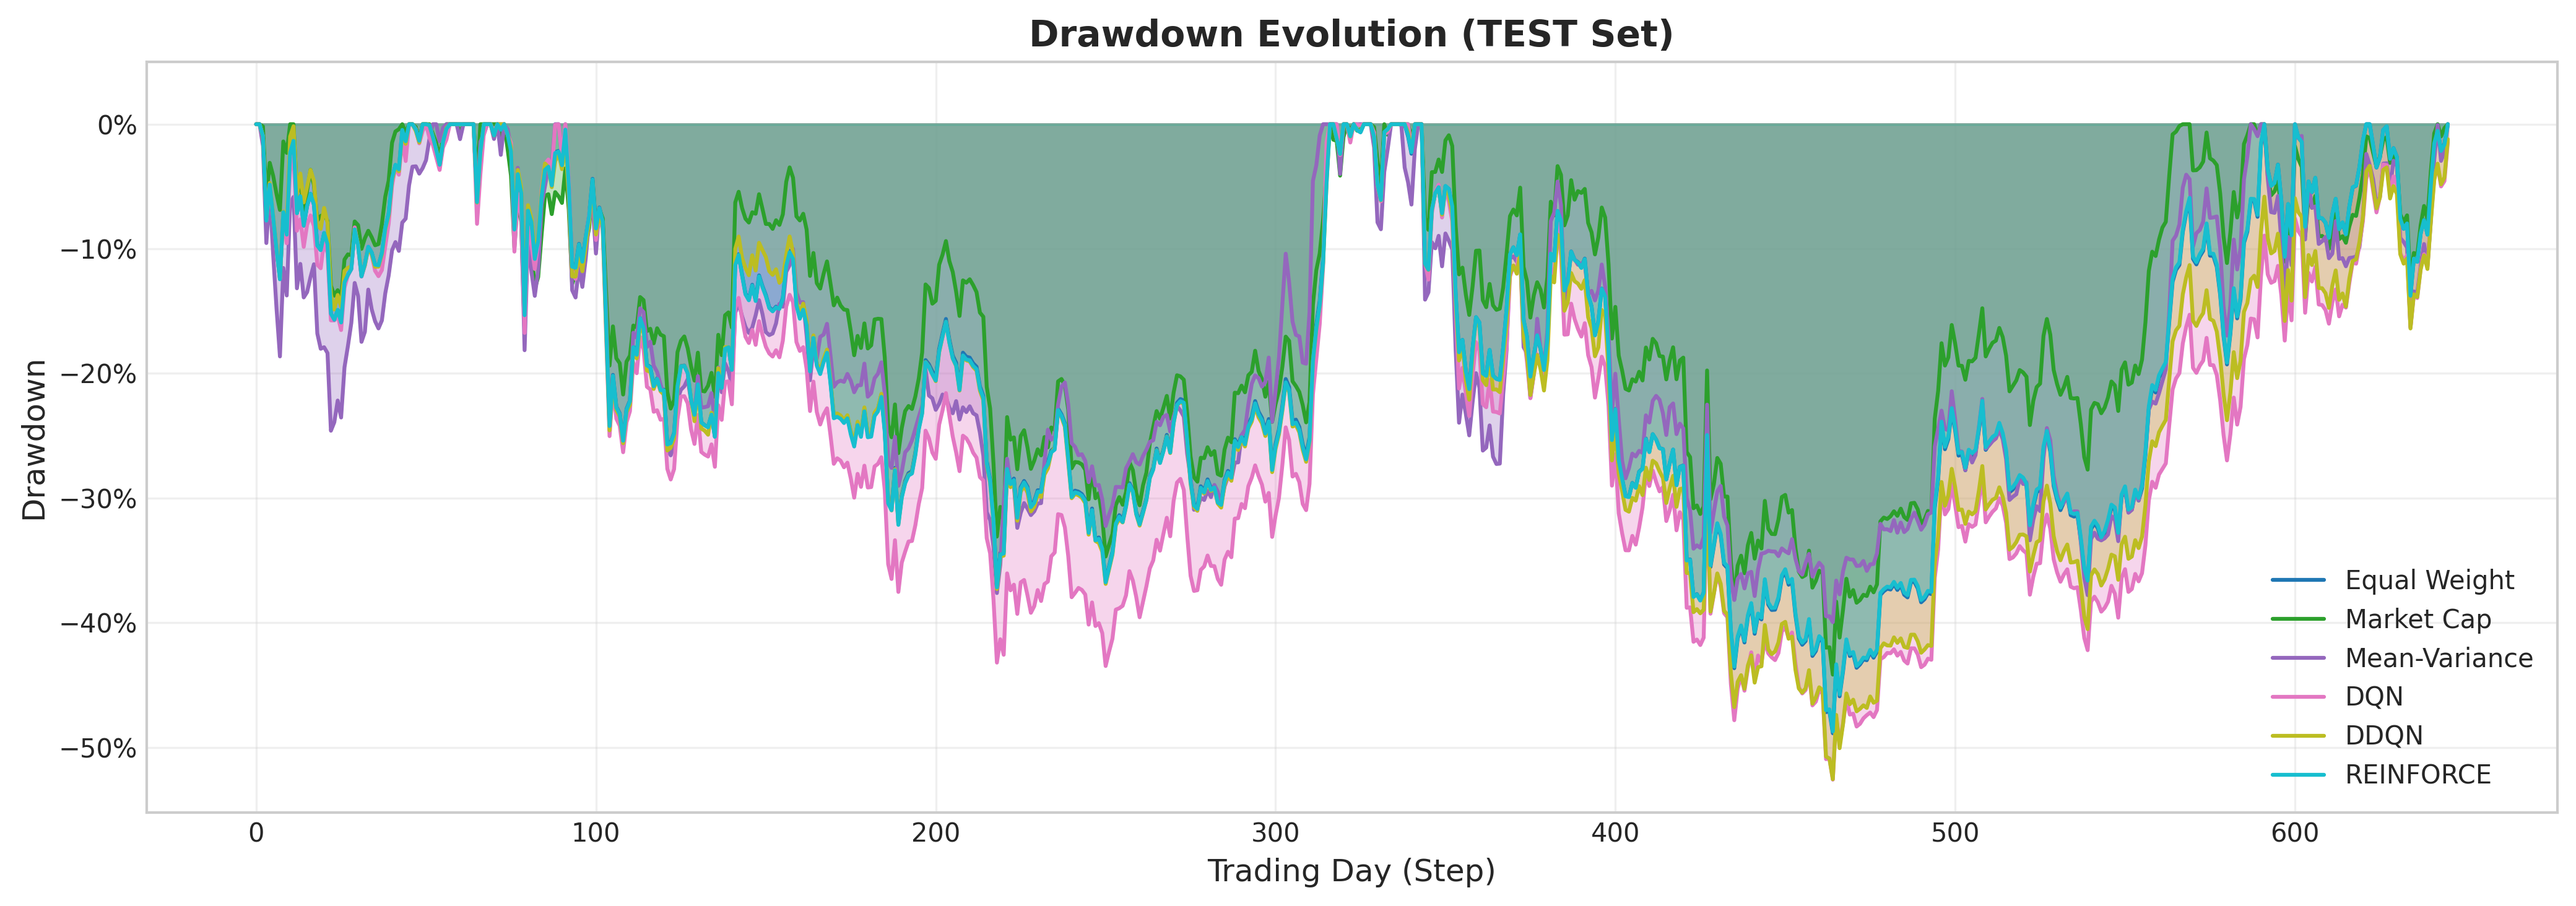
\includegraphics[width=\textwidth]{figures/drawdown.png}
    \caption{Drawdown analysis over the test period. Despite achieving the highest returns, Mean-Variance maintains the lowest maximum drawdown (39.96\%). The value-based RL agents (DQN, DDQN) experience the deepest drawdowns ($>$52\%).}
    \label{fig:drawdown}
\end{figure}

% Rolling Sharpe figure
\begin{figure}[htbp]
    \centering
    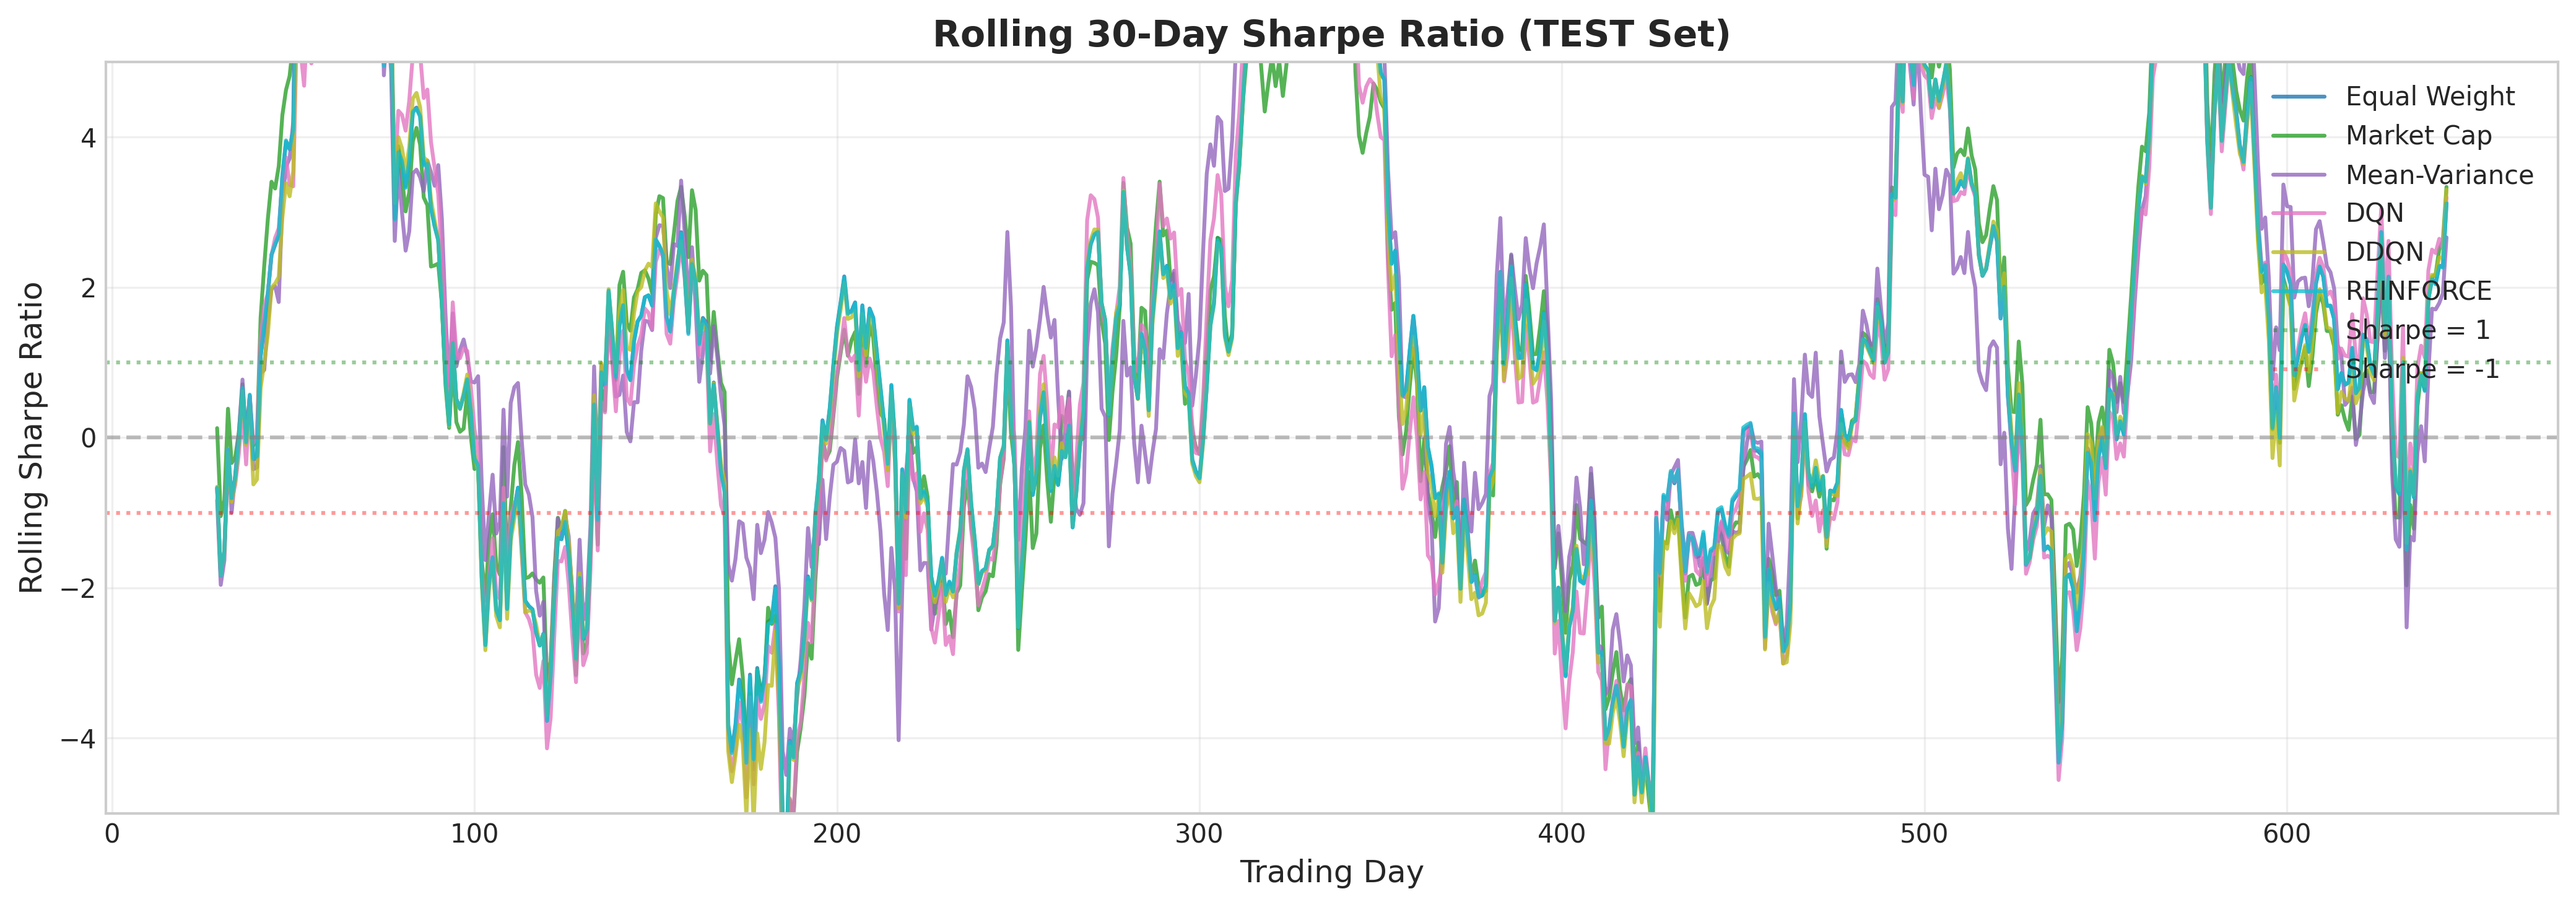
\includegraphics[width=\textwidth]{figures/rolling_sharpe.png}
    \caption{Rolling 60-day Sharpe ratio over the test period. Mean-Variance consistently maintains the highest risk-adjusted performance. All strategies show significant Sharpe ratio variation across different market regimes.}
    \label{fig:rolling_sharpe}
\end{figure}

% Allocation comparison figure
\begin{figure}[htbp]
    \centering
    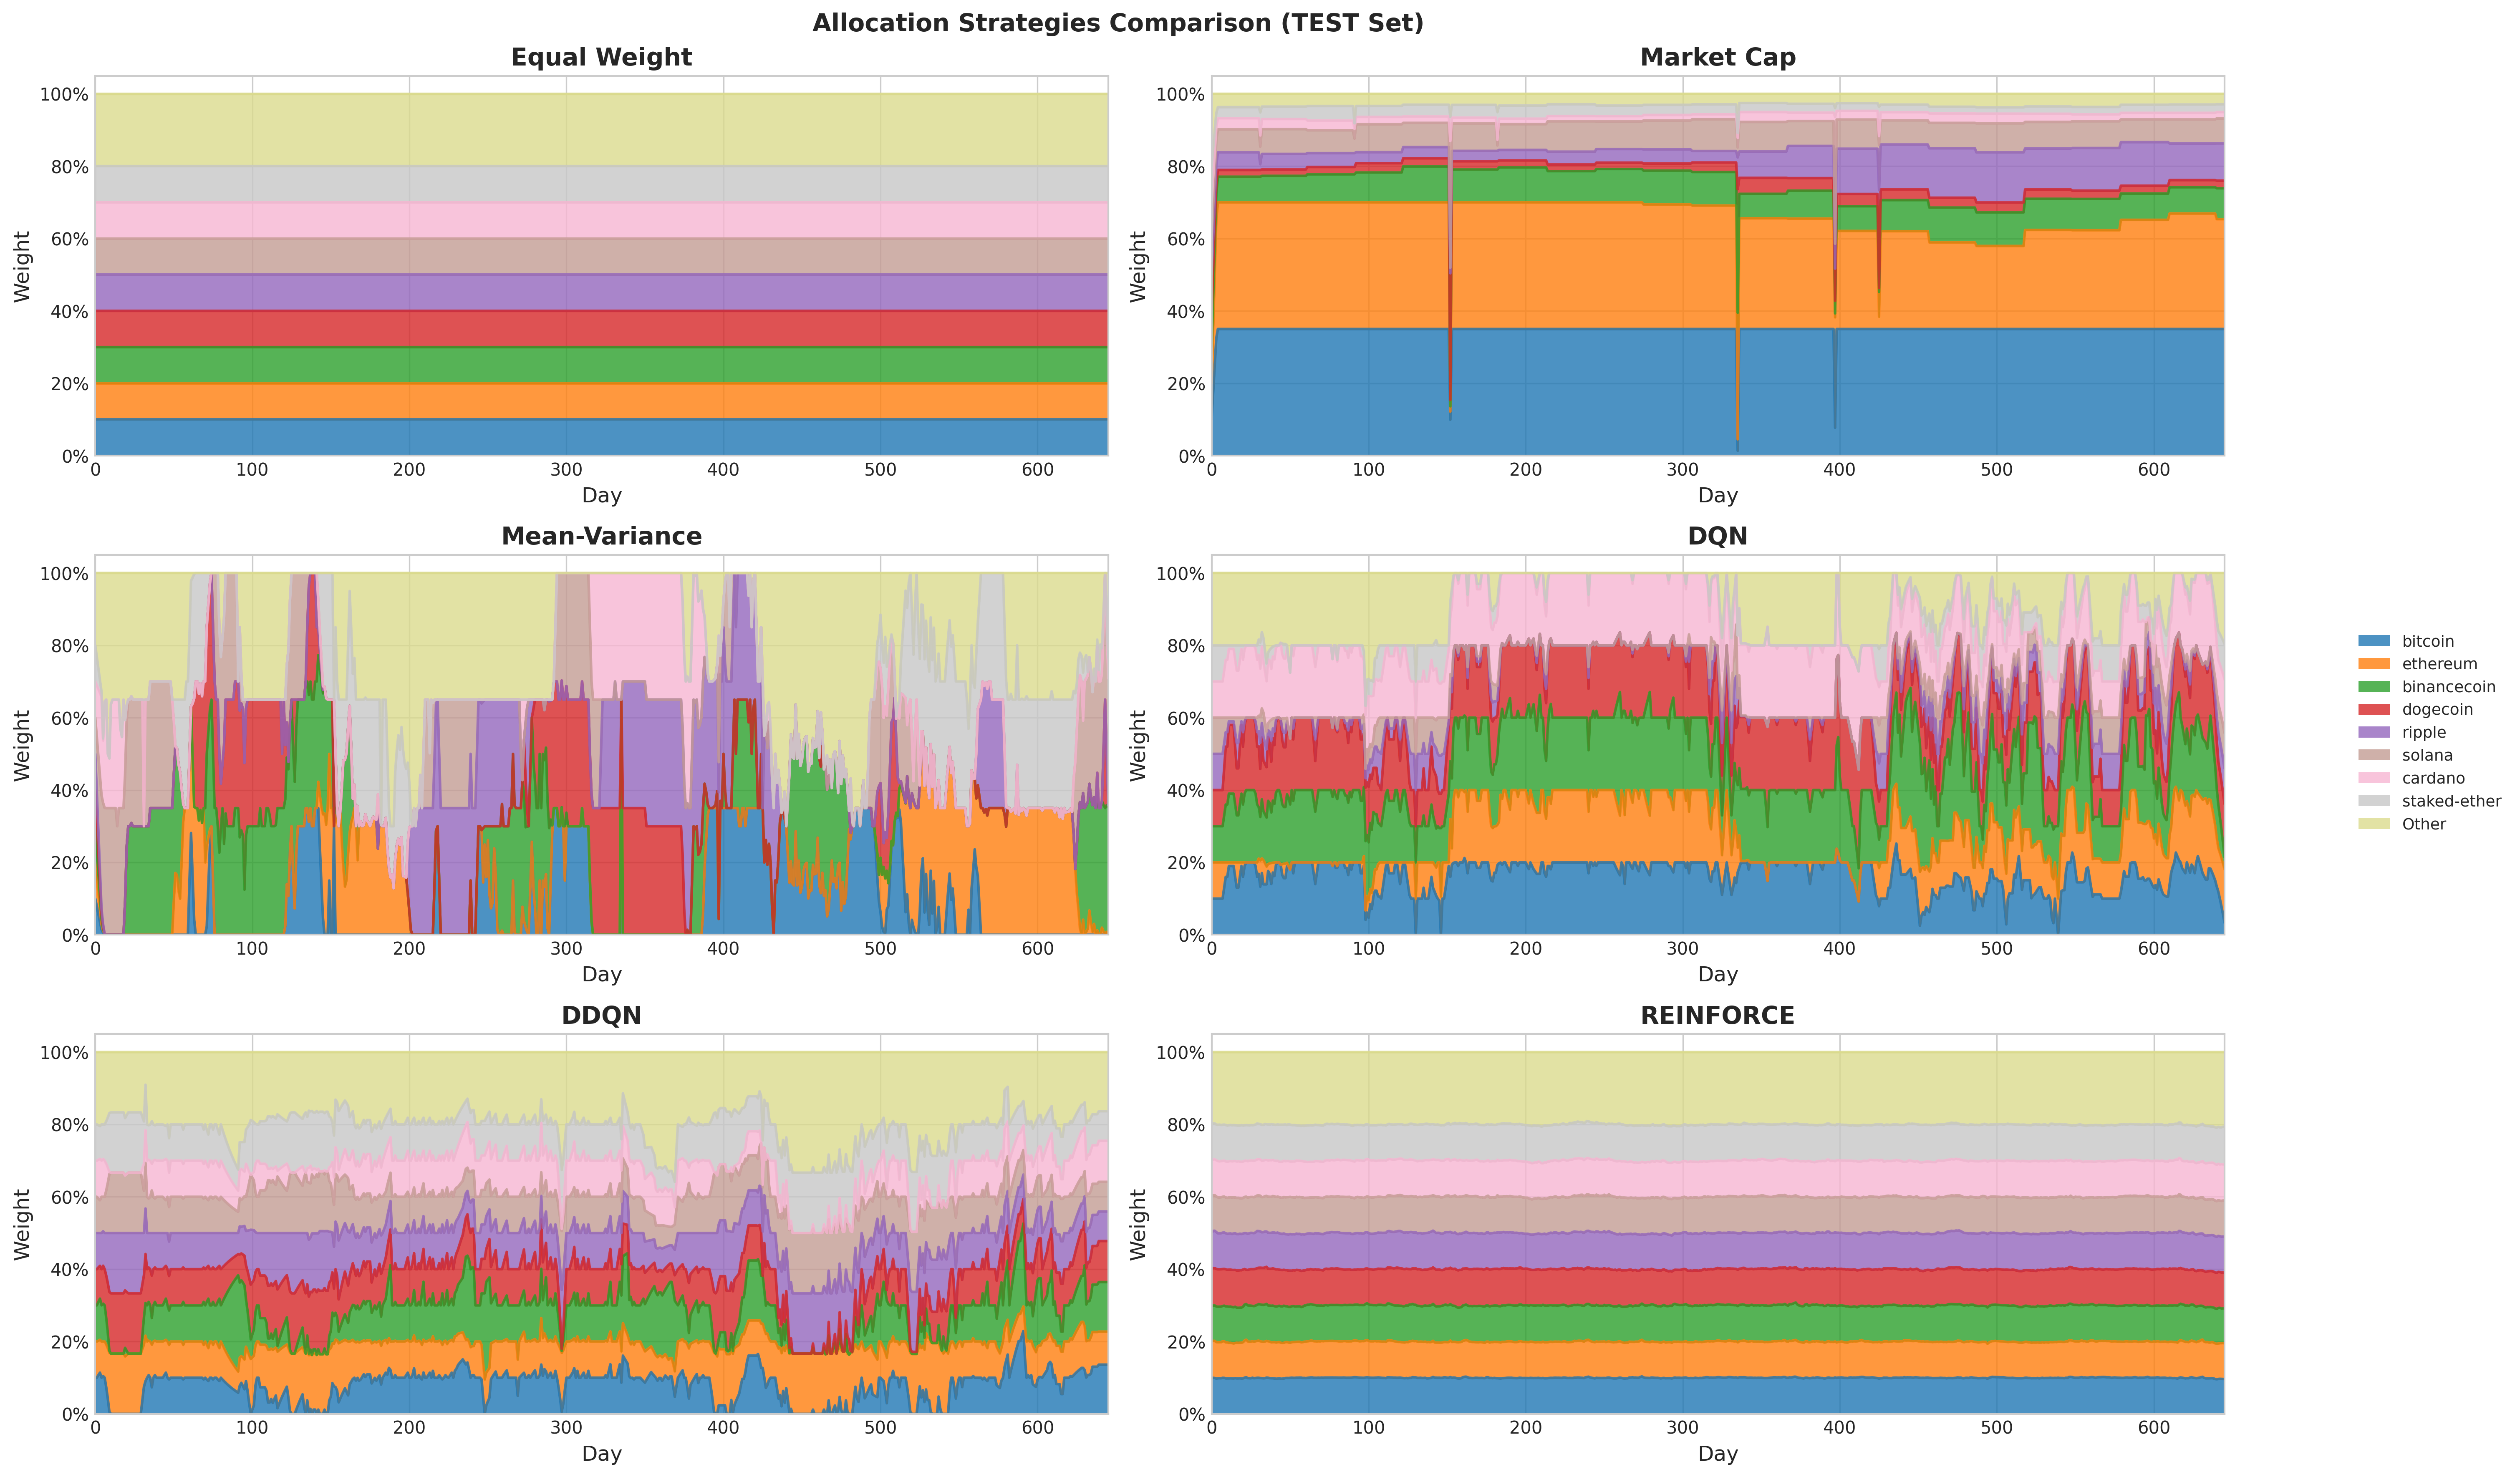
\includegraphics[width=\textwidth]{figures/allocation_comparison.png}
    \caption{Portfolio allocation comparison across strategies over the test period. Mean-Variance exhibits dynamic reallocation with concentrated positions, while Equal Weight maintains uniform distribution. REINFORCE closely mirrors Equal Weight behavior with near-uniform allocations, whereas DQN shows more active rebalancing with concentrated positions in select assets.}
    \label{fig:allocation_comparison}
\end{figure}

\paragraph{Key Observations.} Mean-Variance achieved the highest returns among all strategies, more than double that of the next-best strategy (366.54\% vs.\ 168.50\%), while simultaneously maintaining the highest Sharpe ratio (1.640) and the lowest maximum drawdown (39.96\%). This suggests that during our test period, historical return and covariance estimates provided genuinely useful predictive signal for cryptocurrency markets---a finding that warrants further investigation given the efficient market hypothesis often assumed in academic finance.

Among the reinforcement learning agents, REINFORCE achieved performance nearly identical to the Equal Weight baseline (166.98\% vs.\ 168.50\% return, 1.212 vs.\ 1.217 Sharpe), suggesting the learned policy converged toward a passive, low-turnover strategy. The allocation comparison in \Cref{fig:allocation_comparison} confirms this interpretation: REINFORCE maintains near-uniform allocations virtually indistinguishable from Equal Weight, indicating the policy gradient learned to minimize transaction costs rather than exploit predictive signals in the observation space.

The value-based agents underperformed all baselines. Both DQN (155.47\%) and DDQN (144.50\%) achieved lower returns than Equal Weight, Market Cap, and Mean-Variance. Their elevated turnover rates (10.88\% and 8.39\% respectively) suggest that the delta-based action space, while intuitive, encouraged excessive rebalancing that transaction costs ultimately penalized. Moreover, contrary to expectations from the broader RL literature~\citep{vanHasselt2016ddqn}, Double DQN performed worse than standard DQN in this domain; the reduced Q-value overestimation did not translate to improved portfolio performance.

Examining the turnover-return relationship more broadly, lower-turnover strategies (Equal Weight: 0.25\%, REINFORCE: 0.82\%) achieved competitive returns, while high-turnover strategies incurred significant transaction costs. Mean-Variance stands as the notable exception where active rebalancing generated substantial value, achieving 13.50\% daily turnover alongside superior risk-adjusted returns. The allocation dynamics in \Cref{fig:allocation_comparison} reveal that Mean-Variance dynamically shifts between concentrated and diversified positions based on rolling covariance estimates, while DQN frequently concentrates positions in select assets before rapidly rebalancing, explaining its high turnover without commensurate performance improvement.
